% TeXShop auf xelate und Unicode UTF 8 einstellen
%!TEX TS-program = xelatex
%!TEX encoding = UTF-8 Unicode

%% Store loaded files into log
\listfiles

%% Präambel
\documentclass[fontsize=16pt]{scrreprt}
%% Will Robertson's fontspec.sty zum Einbinden von Systemschriften verwenden
\usepackage{fontspec,xltxtra,xunicode}
\defaultfontfeatures{Mapping=tex-text}
%% Text in den Absätzen in der seltsamen Schreibschrift setzen
\setromanfont[Mapping=tex-text]{Noteworthy}
%% Überschriften im heidnisch angehauchten Stil verfassen
\setsansfont[Scale=MatchLowercase,Mapping=tex-text]{SignPainter}
%% Ich bezweifle zwar, Monospaces zu benötigen, aber falls doch soll sie halbwegs hübsch sein
\setmonofont[Scale=MatchLowercase]{Andale Mono}

%% Darstellung der automatisch generierten Informationen gemäß neuer deutscher Rechtschreibung
\usepackage[ngerman]{babel}
%% Zitate hübsch machen
\usepackage[german=swiss]{csquotes}

%% Import von PDF Dateien, und zwar seitenweise.
\usepackage{pdfpages}

%% Import von Grafiken wie JPG und PNG
\usepackage{graphicx}

%% Hyperref für dokumentinterne Verknüpfungen
\usepackage{hyperref}

%% Metainformationen über das Dokument
\title{Sonor, Sandläufer der Tarr}
\author{Marco Feltmann}

%% Datei dazu ermuntern einen Index für das Inhaltsverzeichnis zu verwalten
\makeindex

%% Neudefinition von \emph in fett weil Noteworthy leider keinen italic Schriftschnitt besitzt
\let\emph\relax % there's no \RedeclareTextFontCommand
\DeclareTextFontCommand{\emph}{\bfseries\em}

%% Dokument beginnen
\begin{document}

%% Titelseite aus eigenes PDF einbinden
\begin{titlepage}
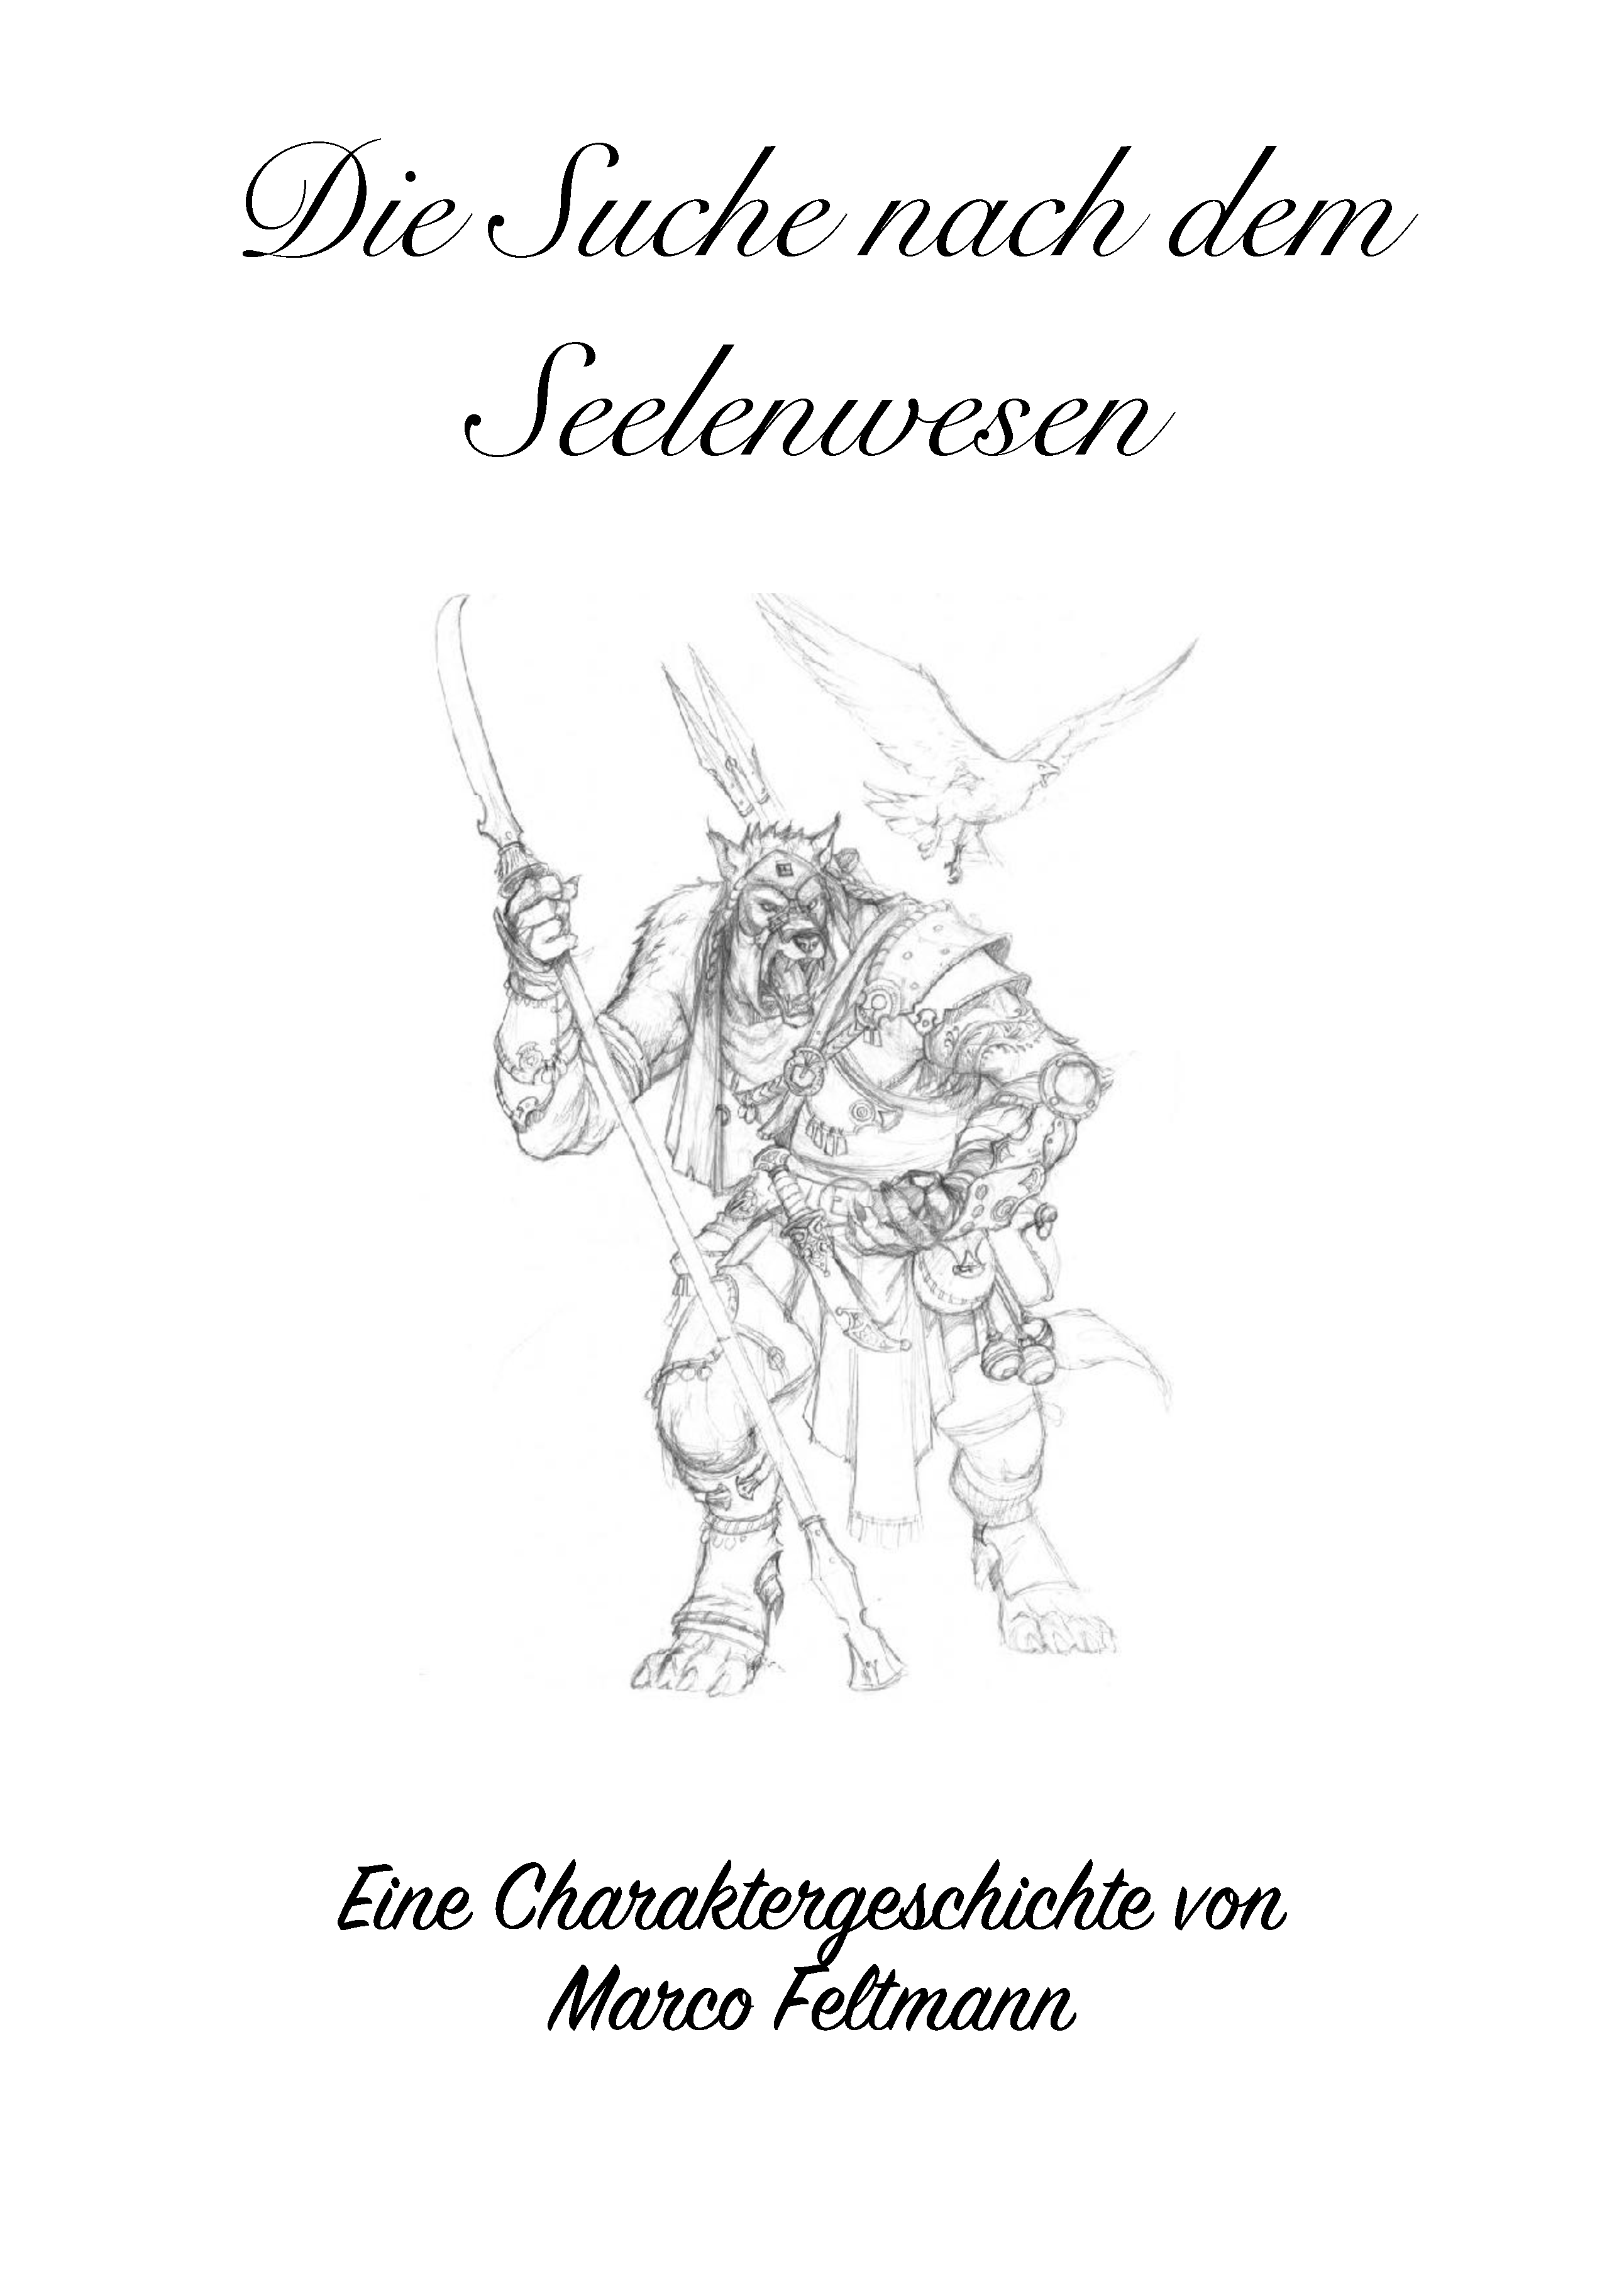
\includepdf{Images/titlepic.pdf}
\end{titlepage}

%% Inhaltsverzeichnis direkt hinten dran
\tableofcontents

%% Reihenweises Einbinden der einzelnen Kapitel
\part{Vorgeschichte}
	Ungefähr 16 Jahre vor den in dieser Chronik aufgezeichneten Abenteuern war es eine schwere Zeit in der Wüste Surmakar. Zugegebenrmaßen gab es in Surmakar selten einfache Zeiten, Schwierigkeiten waren der übliche Zustand in dieser Umgebung und daher nichts Verwunderliches. 
	Unüblich hingegen war die Tatsache, dass das leitende Tarr-Paar in diesem Jahr keinen Welpen gebar, so dass das Privileg der Stammeserhaltung an die in der Rangordnung direkt unter ihnen angesiedelte junge Familie ging.
	
	Sonor sollte der erste Welpe dieses Stammes werden, der nicht die Privilegien der Leit-Tarr hatte, sondern als Sohn zweier Schwarzkamelzüchter aufwuchs.

	
	\section{Frühe Kindheit}
	
	\section{Jugend}
	
	\section{Der Weg des Sandläufers}
	\subsection{Schicksalhafte Begegnung}
	Auf einer seiner Jagden zur Übung und Orientierung fand er auf einem Felsen liegend eine Gestalt, kaum einen viertel Meter lang und dünn wie eine Kralle. Diese Schlange mit rotbraunem Schuppenkleid und sandfarbener Bauchseite wirkte auf ihn wehrlos.
	Als er sie so ansah, hörte er seinen Großvater ihn auffordern, das Tier zu füttern damit es wieder zu Kräften komme.
	Er kniete sich auf ein Bein ab, umgriff vorsichtig das Wesen, welches zwar auf ihre Art energisch protestierte, sich aber mitnehmen ließ.
	
	Bei dieser Jagd konzentrierte sich Sonor auf kleinere Lebewesen wie Wüstenmäuse und Eidechsen. Es fiel ihm schwer diesen winzigen Spuren zu folgen, doch war ihm bewusst, dass auch das Aufspüren und Verfolgen kleinster ungenauester Spuren eine Grundvoraussetzung für jeden Sandläufer ist.
	
	Als er abends zum Lagerplatz zurückkehrte, hatte er einen Geier für den Stamm besorgt und begann, sein Mündel die erlegten Kleintiere zum Fraß zu reichen und eine kleine Schale mit Wasser neben sie zu stellen. 
	
	\subsection{Ein zwielichtiger Händler}
	Niemand in seinem Stamm schien sich so richtig für seinen Fund zu interessieren, der nun mittlerweile durch gute Fütterung fast 30cm lang und so dick wie sein Zeigefinger war.
	Mittlerweile hatte er sich einen weiteren Lederbeutel gefertigt, in den er sie packte wenn eine Jagd bevor stand.
	
	Nach langer Zeit kreuzte ein fahrender Händler den Stamm und versuchte seine Waren feil zu bieten.
	Sonor hatte eigentlich nichts für den Ramsch übrig und die übrigen Stammesmitglieder beschwerten sich über die unerhört hohen Preise, dennoch ging er hin und hielt Ausschau nach irgend einem Utensil für \enquote{Wadjet}, wie er seine Begleitung auf Geheiß der ersten Stammesführerin nannte.
	Als ihm nicht so recht einfiel was er kaufen sollte, fragte er den Händler direkt nach einer Empfehlung.
	Dieser schien spontan sehr freundlich zugetan und wollte das Tier einmal sehen, um sich einen Überblick über die Größe zu machen. Schließlich wolle er das perfekte Ding für sie heraussuchen, so waren zumindest seine Worte.
	
	Sonor reicht ihm Wadjet und wundert sich noch, warum der Händler das Tier so weit in der Mitte greift und wieso er versucht sie in einen Jutebeutel zu stecken. 
	Einen Transportbeutel hatte er doch schon für sie und seiner Einschätzung nach war Leder um Längen besser geeignet als Stoff.
	Bevor er Zeit hatte zu überlegen was hier eigentlich gerade passierte, biss Wadjet dem Händler bereits kräftig in den Muskel zwischen Daumen und Zeigefinger der linken Hand. Aufschreiend ließ dieser das Tier fallen, welches sich sofort auf Sonor zu schlängelte und sich in den Lederbeutel heben ließ.
	
	Der Händler wickelte schimpfend und keifend den Beutel um die Bisswunde, wobei sie für Sonor wirklich harmlos aussah. 
	Das Leitpaar konnte den Händler nur mit viel Mühe davon überzeugen, die Weiterreise erst am späten Nachmittag anzutreten statt sofort in die Mittagshitze zu starten.
	Dem Mann ging es mit voranschreitender Zeit zusehends schlechter. 
	Obwohl die Bisswunde mittlerweile fast zwei Stunden alt war und bereits zu bluten aufgehört hatte, fing sie plötzlich und unvermittelt wieder an.
	Die Blutung aus der Hand wurde mit der Zeit so stark, dass jeder Verband innerhalb von Minuten komplett getränkt war. 
	Zusätzlich traten im zu späterer Stunde, an eine Weiterfahrt war in seinem Zustand nun gar nicht mehr zu denken, auch noch aus Nase, Ohren, Augen und Mund Blut aus.
	Einige Mitglieder des Stammes behaupten gesehen zu haben, dass sogar seine Hose am Hintern voller Blut war, als sich der Händler einmal drehte um an dem Blut nicht zu ersticken.
	
	Der Stamm pflegte den Händler, versorgte dessen Kamele und hielt zusätzlich noch den Stammesbetrieb so gut es eben ging aufrecht. Der Zustand des Erkrankten besserte sich nicht. Die Bissstelle sah mittlerweile merkwürdig verfärbt aus und Daumen sowie Zeigefinger der linken Hand waren stark angeschwollen und komplett schwarz geworden.
	Auch bekam der Mann am ganzen Körper Blutergüsse unter der Haut, so als schlage eine unsichtbare Macht wahllos auf ihn ein.
	Mit seinem Verstand schien es auch nicht mehr so weit her. 
	Er betete zu den unterschiedlichsten Göttern sie mögen ihm seine Verhandlungstaktiken doch vergeben und ihn erlösen von diesem Leiden.
	Sonor missfiel die Wortwahl des Fremden. 
	So unpräzise Wünsche konnten zu einer Erfüllung führen, die eventuell nicht so ganz dem entsprechend, wie der Wünschende sich das eigentlich gedacht hatte.
	 
	Er sollte Recht behalten. 
	Nach mehr als fünf Tagen und Nächten voller Blut, unzähliger zusätzlicher Blutergüsse und sogar einer offenbar gelähmten Körperhälfte starb der Mann im Stammeslager. 
	Getreu ihren Prinzipien haben die Stammesmitglieder den Händler ehrenvoll beigesetzt.
	Als es dann an die Aufteilung der Besitztümer ging, wurden alle Lebensmittel des Mannes beseitigt. 
	Es sah zwar wie eine überirdische Macht aus, die ihn geißelte, aber Sicherheit geht in der Surmakar vor.
	Wer weiß, ob nicht ein vergiftetes Lebensmittel derartige Auswirkungen haben kann. 
	

	\subsubsection{Referenzen aus der Anderswelt}
	
	Gemäß Wikipedia wird das Gift der Ägyptischen Sandrasselotter, welche Wadjet zum Vorbild stand, wie folgt beschrieben:
	
	\begin{quotation}
		\texttt{Alle Sandrasselottern besitzen ein hochpotentes Schlangengift. Das Gift enthält	unter anderem ein hochwirksames Hämotoxin (Blutgift) und ein weniger wirksames Neurotoxin (Nervengift). Für die Störung der Blutgerinnung ist das Enzym Ecarin verantwortlich. Das Gift ist im Kreislaufsystem sehr stabil, sodass die	Ungerinnbarkeit des Blutes über Wochen hin anhalten kann. Nach einem Biss kommt es innerhalb von ein bis sechs Stunden zu unstillbaren Blutungen aus der
		Bisswunde sowie über die Schleimhäute, wodurch Blut aus Nase, Mund und Darm
		austritt. Die Haut färbt sich um die Bissstelle herum. Das gebissene Glied
		schwillt extrem an und es entstehen Nekrosen. Weitere Folgen können
		Bluterbrechen, blutiger Speichel und Blutergüsse unter der Haut, sowie
		Herzrhythmusstörungen, Blutdruckabfall, Hirnblutungen und Nierenschäden sein. Es
		können auch Lähmungserscheinungen und ein Schockzustand auftreten. Ohne
		Antise rumbehandlung kommt es in den meisten Fällen zum Tode.}

		\texttt{Gegen das Gift der Ägyptischen Sandrasselotter gibt es kein spezielles Antiserum (Antivenin), bei einem Biss wird entsprechend ein allgemein bei Echis-Arten	nutzbares Mittel eingesetzt.}
\end{quotation}

\section{Die Bitte des Ältesten Geistheilers}
Es ist ein grauer Tag für den Ältesten Geistheiler des Stammes. Seit Tagen schon sagen Wind und Wolken der Surmakar ein schlechtes Omen voraus, doch er kann es einfach nicht deuten. Auch die Geister der Ahnen beantworten ihm seine Fragen nicht.

In Abstimmung mit den Stammesführern wird ein Wettkampf unter den jungen Vargen des Stammes ausgerufen, bei dem Zuverlässigkeit und Zielstrebigkeit der einzelnen Persönlichkeiten geprüft wird. 
Auf Grund seiner in der Saundläuferausbildung erworbenen Fähigkeiten kann Sonor diesen Wettkampf knapp für sich entscheiden.

So wird er nun mit einer ausreichenden Reisekasse nach Ioria geschickt, dem Orakel die Zeichen zu erläutern und nach deren Bedeutung zu fragen.
Dies nicht nur Sonors Chance, seine Wichtigkeit in der Gruppe zu demonstrieren, sondern liefert auch noch die Möglichkeit eine Höhere Macht nach dem Aufenthaltsort seines Seelentiers zu befragen.

Voller Vorfreude macht Sonor sich auf die Reise nach Ioria.

\part{Der Chroniken erster Teil}
Die Reise mit dem Schiff von Surmakar bis Ioria dauert dem jungen Vargen viel zu lange. 
Vor Allem stellt sich die Fahrt für ihn, der nur Sandmeere und Dünen kennt, als sehr eintönig und unliebsam heraus.
Das Auf und Ab des Schiffes in den Wellen erinnert ihn ein wenig an das Geschaukel auf den Schwarzkamelen, die er als junger Welpe geritten war, bevor das Missgeschick mit seinen Klauen passierte.
Allerdings brachte die Unruhe der Kamelreise ihn von allein auf den Gedanken, dass die Fortbewegung zu Fuß die einzige von der Natur vorgegebene Art und Weise des Reisens sei.
Diese Schifffahrt festigt seine Meinung diesbezüglich noch weiter.
 
Nach einer gefühlten Ewigkeit kann Sonor endlich den Hafen Iorias sehen.
Gespannt wartet er auf die Ankunft des Schiffes und brennt voller Eifer darauf, den Auftrag auszuführen und das Orakel wegen der Zeichen der Wüste zu befragen, zu denen sich die Geister der Ahnen so beharrlich ausschwiegen. Selbstverständlich brennt auch sein eigenes Ziel in ihm und er hofft auf einen Fingerzeig zum Lebensraum seines Geisttieres.

Vom Hafen ist es noch ein Stück in die Stadt. Der Boden sagt seinen Füßen überhaupt nicht zu, er ist viel zu hart und viel zu kalt. 
Wobei die Behauptung \enquote{zu kalt} für das gesamte Areal hier zutrifft.
Interessiert blickt er sich auf dem Weg in die Stadt um. Kreaturen unterschiedlichster Art und Abstammung tummeln sich auf den Straßen, ihre Kleidung so verschieden wie ihre Herkunft. Ihm wird klar, dass er sich hier an einem zentralen Punkt befindet, der die reisenden Händler zu ihren Erzählungen anregt und die unterschiedlichen Wesen Lorakis' hier zusammen führt. 


\chapter[13. November 2016]{Ioria}
\begin{center}
\enquote{\emph{Ioria} -- der Nabel der Welt. Die Orakelstadt. Der Sündenpfuhl.}
\end{center}

\section{Seltsame Resonanzen}
Wenige Schritte nachdem Sonor den Hafen verlassen hat und sich interessiert umschaut, passiert etwas sehr merkwürdiges. Die Welt um ihn herum scheint für den Bruchteil einer Sekunde völlig still zu stehen. Alle Farbe scheint aus den umgebenden Wesen heraus gewaschen und sie verschwimmen fast vor seinen Augen. Er hört eine schwache Melodie klingen.
Lediglich eine dunkel gekleidete Gestalt mit unter einer Kapuze verborgenem Gesicht sticht scharf aus der Umgebung hervor und scheint vom Stillstand nicht betroffen.

Kaum ist dieses seltsame Gefühl vorüber, wird Sonor von hinten angerempelt. Offenbar war ein drittes Wesen an dieser Erfahrung beteiligt, welches er allerdings nicht sehen konnte, da sie hinter ihm stand.

\subsection{Lian, feurige Albin des Phoenixordens}
Die Gestalt, die den Varg angerempelt hatte, ist nur etwa 30 Zentimeter kleiner als er. Auffällig an ihr ist\ldots Nun, eigentlich alles. Blasse Haut, rotbraunes Haar, rote Augen, roter Schuppenpanzer, eine rote Insignie mit Ähnlichkeit eines brennenden Vogels. Weiterhin trägt sie ein Schwert mit sich herum.

Nach eigenen Angaben möchte sie den hiesigen Orden ihrer Religion besuchen. Irgendwas mit Fennex oder so. 

\subsection{Volton, alchemiekundiger Mensch}

Der auffallend kleine Mensch wirkt sehr ausweichend und scheint sich in seinem Kapuzenmantel zu verstecken. Eventuell möchte er seine seltsamen unterschiedlichen Augen verbergen, eines weiß, das andere rot. Insgesamt ist er mit Rucksack und Stab ziemlich bepackt und wird von einer schwarzen Krähe begleitet.

\section{Eifriger Eber}

Nach einer kurzen Rücksprache mit den Geistern der Ahnen folgt Sonor den beiden Fremden in die Stadt.


Die Gruppe kehrt im Gasthof \enquote{Eifriger Eber} ein, worauf Volton die Aufmerksamkeit aller Anwesenden auf sich zieht. Zu Sonors Überraschung wird die auffallend rote Lian nur ganz kurz beäugt und er selbst überhaupt nicht wahrgenommen.

Der übertrieben freundliche Gastwirt nimmt die Bestellung der Gruppe auf und die drei nutzen die Wartezeit einander vorzustellen.

Lian und Sonor haben das gleiche Ziel: Das Orakel. Volton beschließt die Beiden zu begleiten, um das Orakel nach dem jüngsten Ereignis zu befragen.
Lian sieht dem längsten Aufenthalt entgegen, da sie noch Aufgaben für ihren Orden in Ioria erledigen möchte.
Sonor stuft sie als eine Art Geistheilerin ein, die anstatt mit ihren Ahnen mit ihrem Fönicks spricht. 

Nach dem Essen begeben sich die drei zur Ruhe, nachdem sie der vehementen Einladung der letzten drei Gäste nicht nachkommen.
Sonor lässt sich im Gemeinschaftsschlafsaal nieder während Volton und Lian jeweils ein Einzelzimmer beziehen.
Für Sonor gestaltet sich die Wahl des Gemeinschaftszimmers als ausgesprochen nachteilig, da sich zu später Stunde vier grölende und lärmende stark angetrunkene Gäste ebenfalls im Gemeinschaftssaal niederlassen.

\section{Ärger in der Stadt}

Obwohl der Lärm, den diese Kerle produzierten, Sonor den erholsamen Schlaf versagten, fühlt er sich am nächsten Morgen nicht übermäßig gerädert.

Volton und Lian sitzen bereits unten und haben sich von der Wirtin Frühstück bringen lassen. Die Wirtin scheint Lian sehr zugetan zu sein. Sonor verabschiedet sich aus der Ferne, da er früh zum Orakel aufbrechen will. Gerade im Begriff die Tür zu öffnen rempelt ihn ein Mensch in weißer Uniform fast um, als dieser hinein stürmt und Volton wegen Kindesentführung als verhaftet bezeichnet.
Einer Eingebung folgend schließt Sonor die Tür von innen und versperrt diese.

Lian scheint unerfreut über diese Unterbrechung und dem Varg fällt auf, dass um ihre Hand rote Funken auflodern.
Nach längerem Hin und Her, in der sich der Weiße mal im Nachteil, mal im Vorteil wähnt, lässt Sonor dann den Rest der Truppe in die Taverne.
Ein offenbar ranghöherer Weißer erklärt ihnen, dass lediglich ein dem Protokoll entsprechendes Verhör statt finden wird, da man Volton die Vorgehensweise der Zutrittsbeschaffung nicht zutraut.

Von den vier anderen Gästen fehlt jede Spur, die Wirtin beteuert allein mit ihrer Tochter den Eber zu führen und stellt fest, dass auch ihre Tochter offenbar verschwunden ist.

Nachdem Volton noch irgend einen Brief an irgend einen Mentor geschrieben hat, begeben sich die drei mit auf die Wache.

Das Abgeben der Waffen am Empfang scheint für Lian ein regelrechtes Problem zu sein, was Sonor überhaupt nicht nachvollziehen kann. Erst als ein älterer Herr mit Schildkröteninsignie in den Raum tritt und ihr versichert die Waffe wie seine Eigene zu hüten, entspannt sie sich sichtlich. Das heißt, die Funken um ihre Hand und das Leuchten ihrer roten Augen wird weniger.

Das Verhör wird von einem Vaigarr durchgeführt und ist entsprechend informativ. Nix gesehen, nix gehört, Opfer unbekannt, Tschüss.
Offensichtlich kamen die beiden Anderen nicht so glimpflich davon, da Sonor sehr lange auf die Rückkehr der beiden warten musste.
Ihnen allen wurde mitgeteilt, dass sie bis zur Aufklärung dieser Entführung die Stadt nicht verlassen dürfen.

Der Tag ist bereits voran geschritten und sie stehen nahe am Orakel, so dass Lian sich überreden lässt zunächst das Orakel und erst danach ihren Orden aufzusuchen.

Besagtes Orakel beantwortet die Frage des Ältesten Geistheilers mit einem seltsamen Singsang:
\enquote{Die Schatten heben und senken sich. Die Wüste fürchtet sich. Die Tarr werden bestehen. Die Wüste wird leben.}


\section{Eine neue Aufgabe}

Im Anschluss spricht noch irgend ein Priester mit so einem Schildkrötenemblem mit den Dreien, erzählt irgend eine zusammenhanglose Prophezeiung, sinniert darüber, dass sie zu fünft sein sollten und allerhand ähnlich seltsames Zeug.
Auf Voltons Frage, was das am vorherigen Tag war, benutzte der Mann das Wort \enquote{Splitterträger}. 
Auch er wies darauf hin, dass es sinnvoll sei zunächst in Ioria zu verweilen.

Beim Phönixorden gehen die rätselhaften Ereignisse weiter. Die spartanische Einrichtung und Bewirtung sind das Einzige, mit dem Sonor irgend etwas anfangen kann. Das Gespräch zwischen Liam und einer anderen in noch kräftigerem Rot gekleideten Frau findet in einer Sprache statt\ldots Genau genommen hört es sich für Sonor überhaupt nicht nach einer Sprache an.

Lian klärt sie auf, dass in der Unterstadt Iorias in letzter Zeit viele Kinder entführt wurden. Der Orden beauftragte sie damit, die Täter aufzuspüren und vorzuführen, da sich die seltsamen weiß gekleideten Sicherheitskräfte für die Unterstadt wohl nicht zuständig fühlen.
Weiterhin erzählt sie, dass sie die Namen der jüngsten Opfer bekommen hat und sofort mit der Untersuchung beginnen möchte.

Sonor und Volton willigen ein ihr zu helfen.


\chapter[17. Dezember 2016]{Ioria}
\begin{center}
	\enquote{Die strahlende Metropole im Herzen des Kontinents Lorakis ist das Ziel zahlloser Pilger aus aller Herren Länder.}
\end{center}

\section{Weitere Resonanzen}
\subsection{Niamh, kleine Albin der Straße}
\subsection{Kharr, neugieriger Vaigarr-Kämpfer}

\section{Erste Ermittlungen}



\chapter[14. Januar 2017]{Mondportal}
Der Gnom mit dem Kessel aufm Kopp…

%% Anhänge
\appendix

\newpage
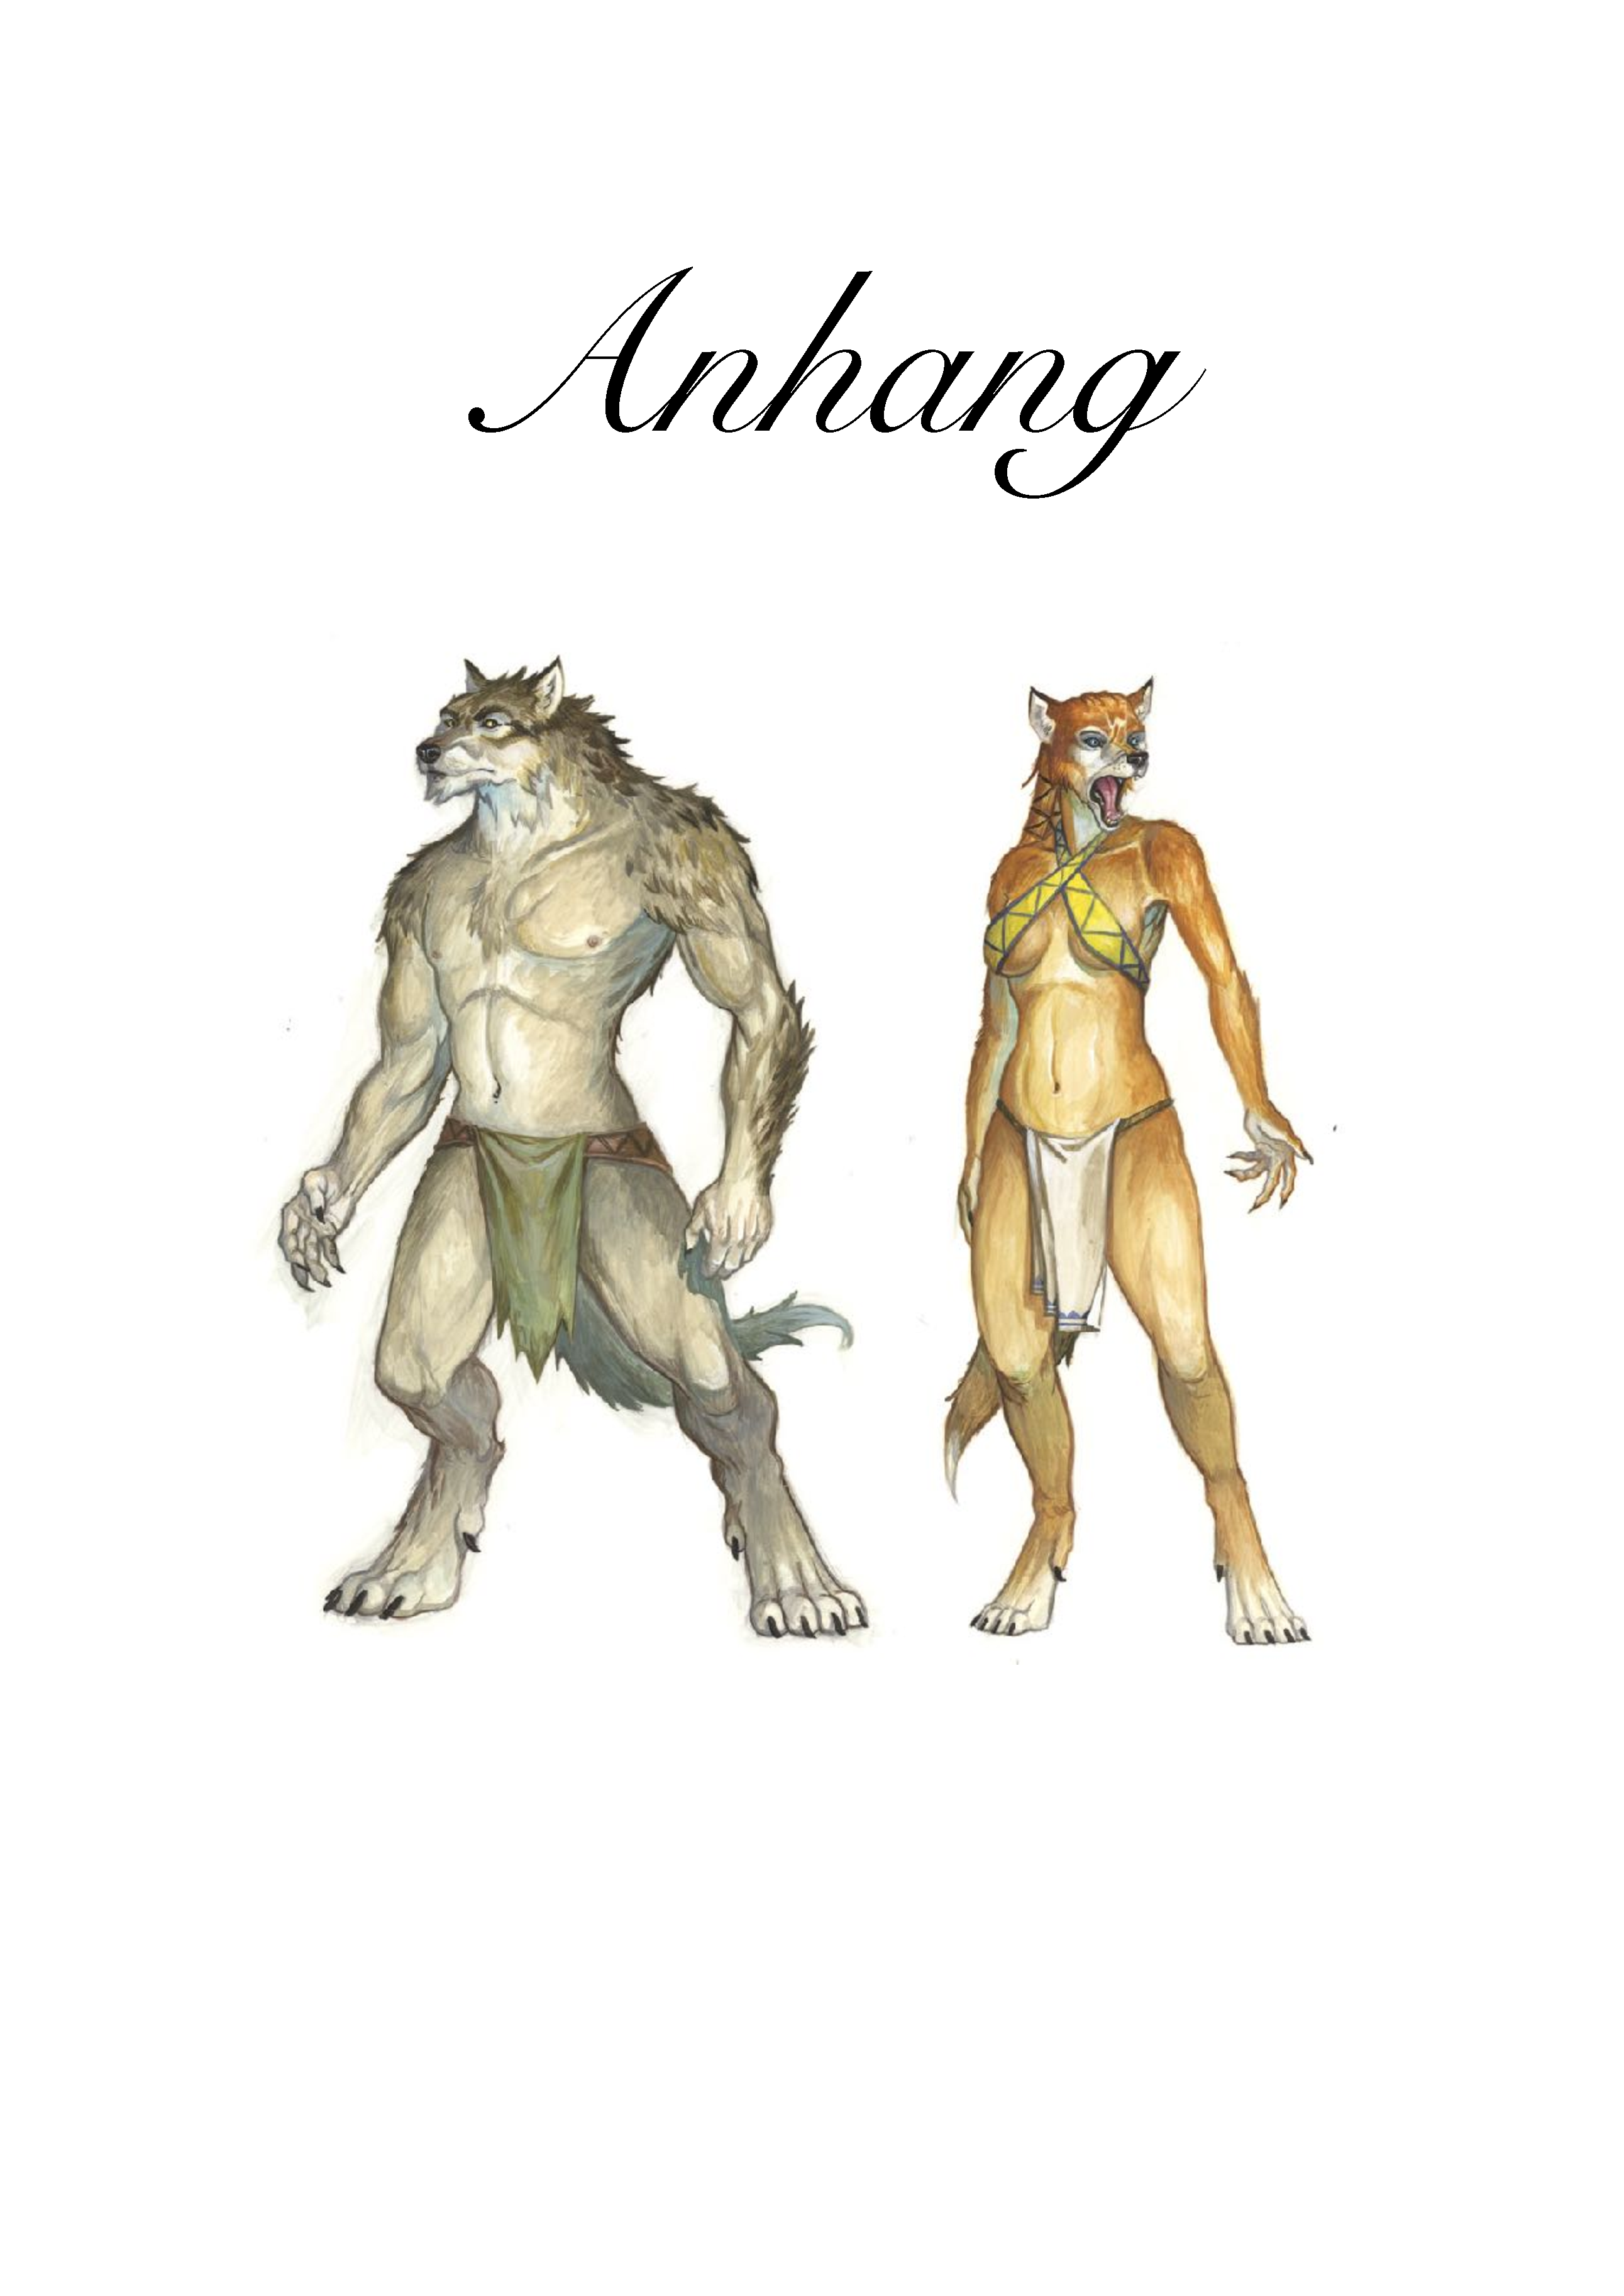
\includepdf{Images/appendixpic.pdf}
\newpage

\chapter{Fragen zum Charakter}

\documentclass{article}

\usepackage[ngerman]{babel}
\usepackage[utf8]{inputenc}
\usepackage[T1]{fontenc}

\usepackage[babel,german=swiss]{csquotes}

\author{Marco Feltmann}
\title{Hilfreiche Fragen für die Ausgestaltung \\ \enquote{Sonor} }

\begin{document}

	\maketitle
	
	\tableofcontents
	
	\section[Aussehen]{Wie sieht der Abenteurer aus, wie wirkt er auf Fremde?}
	
	Sonor ist ein Varg mit sandfarbenem Fell. Trotz
	seiner 2,27 Metern Größe wirkt er mit seinen knapp 125kg Körpergewicht
	verhältnismäßig schmal. Sein Gesicht hat schmale lange Linien, während
	seine dunkelbraunen Augen und seine Ohren unverhältnismäßig groß sind.
	Tatsächlich besteht sein Gesicht zu knapp der Hälfte aus Ohren, so dass
	die verhältnismäßig kleine, kurze und schmale Schnauze kaum auffällt.

	Auch ist sein Gebiss eher zierlich für einen Varg. Zwar sind die Zähne
	scharf und spitz wie bei anderen Vertretern, allerdings hat er
	weniger und sie sind ziemlich kurz.
	Seine Krallen hingegen sind ziemlich beachtlich und gut geschärft. Er
	kann sie im Gegensatz zu den meisten anderen Varg nicht einziehen, da
	sie fest an den Knochen verwachsen sind, was sie allerdings
	widerstandsfähiger macht als bei anderen Varg.

	Gekleidet ist er in braune Wollstoffe mit dunklen Lederapplikationen.
	Auffällig sind die riesigen Waffen, die er mit sich herumträgt. Sowohl
	die Glefe als auch die Speerschleuder sind jeweils über 2 Meter lang und
	umso eindrucksvoller, da Sonor für einen Varg eher schmächtig wirkt.

	Vor Allem abends und in der Nacht fällt dem geneigten Beobachter auf,
	dass aus einem Lederbeutel an seiner Hose ein kleiner, kurzer,
	Kopf herauslugt, der ein wenig wie ein abgerundetes Dreieck aussieht.
	Er gehört zu der knapp 35cm kurzen und schlanken Begleiterin Wadjet,
	deren rotbraunes Schuppenkleid durch einige sandfarbene Flecken
	unterbrochen wird, welche Sonors hauptsächlicher Fellfarbe ähneln.
	Vor Allem vor ihren Ruhezeiten ertönt ein seltsames Gerassel aus dem
	Beutel, das durch die übereinander gleitenden schräg angeordneten und
	gekielten Seitenschuppen Wadjets verursacht wird.

	Sonor selbst wirkt ob dieses bedrohlichen und giftigen Bewohners seines
	Beutels in keinster Weise besorgt. Auf die Frage, ob er keine Angst vor
	Bissen habe, antwortet er nahezu gleichgültig, dass sie das schon oft
	gemacht hat. Es gäbe also nichts zu befürchten\ldots

	Bei spirituellen Anlässen wie der gemeinsamen Jagd mit seinem Stamm
	wählt er immer Kreidestaub und Kohle aus, um sich sein Antlitz im Stile
	seines Schädels zu bemahlen: Der Bereich um die Augen, Lefzen und Ohren schwarz
	(die Nasenspitze ist es ja schon), der Rest weiß mit angedeuteten Zähnen
	auf den Lefzen und zusätzlichen schwarzen Verziehrungen um die Augen und
	Nase.
	
	\section[Soziales Umfeld]{In welchem Umfeld ist der Abenteurer aufgewachsen?}
	
	Sonor stammt aus der Wüste Surmakar, der 'Sonnenweite' und ist das
	einzige Kind einer Familie von Schwarzkamelzüchtern. Bei jedem Zug durch
	die Wüste durfte seine Familie in direkter Nähe von Oasen oder
	Wasserlöchern hausen, da die Kamele ja mit Wasser versorgt werden
	mussten - die Kamelversorgung zählte zu seinen Hauptaufgaben im Stamm.

	Die Oasen waren auch immer die heiligen Stätten des Stammes, da ihre
	Entstehung und Existenz für das Leben in der Sonnenweite essentiell ist,
	ihr Austrocknen dagegen ein untrügliches Zeichen des Vergehens ist.
	
	Sowohl Geburten wie Lebensbundschließungen als auch Einäscherungen wurden immer
	an diesem heiligen Ort in zeremonienartigen Ritualen durchgeführt.


	\section[Beziehungsstatus]{Hat der Abenteurer eine eigene Familie oder eine große Liebe?}

	Sonor hat weder Geschwister noch eine Partnerin. Lediglich seine Eltern
	in Surmakar und sein Stamm sind in seinem Leben wichtig.


	\section[Freund und Feind]{Hat der Abenteurer einen besten Freund und/oder einen ärgsten Feind?}

	Nein.


	\section[Religion]{Zu welchen Göttern betet der Abenteurer?}
	
	Die Religion Sonors Stammes ist kompliziert. Im Prinzip beten sie die
	Geister ihrer Ahnen an und führen ihre Rituale an ihrer Meinung nach magischen
	Orten durch.

	Sonor selbst scheint manchmal Fragen zu murmeln und angestrengt auf
	Antworten zu warten. Ob das seine Art von Gebet ist oder er einfach nur
	introvertiert ist, ist für Dritte schwer zu unterscheiden.


	\section[Magie]{Wie geht der Abenteurer mit Magie um?}

	Sonor führt die Gepflogenheiten seines Stammes fort. Magie wird in
	Ritualen zur Kampfvorbereitung genutzt, um Ausrüstungen zu verbessern,
	die eigenen Kampfreflexe zu stärken oder die erlegten Tiere haltbarer zu
	machen.

	Es ist allerdings sehr verpönt, bei der Jagd direkt mit Elementar- oder
	ähnlicher Magie zu hantieren. Dies erzürne die Ahnen, die den Akt der Jagd an
	sich als Handwerk ansehen, der nur und ausschließlich durch die
	physischen und psychischen Fähigkeiten des Varg vollzogen werden darf.
	Nachweisbare Zuwiderhandlungen werden mit Ausschluss aus dem Stamm geahndet.


	\section[Schicksal]{Wie kam der Abenteurer zum Abenteurerleben?}

	Bei den Sandläufern der Tarr ist es seit je her Tradition, dass der
	älteste Geistheiler des Stammes sie aus ihrem Lehrlingsstand enthoben
	hat. Wie viele vor ihm hat Sonor die Wüste auf der Suche nach dem Wesen
	durchstreift, das seinen Geist erwachsen machen sollte. 

	Nach vielen Jagden, auf deren auch Wadjet ihm begegnete und ihn seither
	beim Erkunden winziger Höhlen und Gänge unterstützt, musste er entmutigt
	feststellen, dass sein Geisttier sich außerhalb der Wüste befindet.

	Sein Mentor gab ihm den Hinweis auf den Weg, dass es die Ahnen erzürne
	Magie zum Aufspüren des Wesens einzusetzen denn das Tier kommt zum Tarr,
	wenn es ihn für würdig hält.

	Die Worte seines Mentoren auf die Goldwaage legend beschloß Sonor, das
	Orakel von Ioria nach dem Gebiet zu befragen, in dieses Tier sich
	aufhält. Schließlich möchte Sonor es ihm so einfach wie möglich machen
	ihn zu finden.


	\section[Antrieb]{Was ist der sehnlichste Wunsch des Abenteurers?}

	Sonor möchte endlich seinen Lehrlingsstatus hinter sich bringen, um
	seinen Stamm sicher durch die Sumarkar leiten und sie mit Nahrung
	versorgen zu können.

	
	\section[Ängste]{Wovor fürchtet sich der Abenteurer am Meisten?}

	Seine größte Angst ist es, das Tier welches seinen Geist erwachsen
	machen soll nicht aufzuspüren. Jeden Tag bittet er seine Ahnen,
	schützend ihre Hände über jenes Wesen zu legen, damit es nicht durch
	unwürdige Lebensformen oder widrige Umstände den Tot findet bevor Sonor
	es gefunden hat.


	\section[Moral]{Wie sehen die Moralvorstellungen des Abenteurers aus?}
	

	Sonor hat kurz nach seinem Aufbruch aus der Surmakar festgestellt, dass
	die Moralvorstellungen seines Stammes nicht unbedingt dem entspricht,
	das andere Völker ausleben. 

	Er ehrt das Leben an sich und als solches, was immer er bekommt teilt er
	unter den Stammesmitgliedern auf, er respektiert das Eigentum Anderer
	und setzt sich nach seinen Kräften für das Wohl seines Stammes ein.


	\section[Frustrationstoleranz]{Wie steht der Abenteurer zu Gewalt und dem Töten von Lebewesen?}


	Leben nehmen um Leben zu erhalten ist in Sonors Welt der einzig richtige
	Umgang mit diesem einmaligen Naturschauspiel. Dies spiegelt sich auch
	den den Jagdritualen wider, in denen nach erfolgreichem Beuteschlag den
	Geistern der Ahnen zu Ehren und Dank ein Fest abgehalten wird.

	Doch auch im Verteidigungsfall, sollte die Auseinandersetzung dem
	Gegenüber das Leben kosten, wird der Leichnam fürsorglich der Obhut der
	Geister der Ahnen übergeben.

	Körperliche Auseinandersetzungen an sich sind allerdings etwas ganz
	Anderes. Sie gehören zum Leben dazu wie das Essen und das Schlafen.
	Wer sich im Recht fühlt und nicht darum zu kämpfen versteht, ist als
	Varg nicht ernst zu nehmen. Wer einer Auseinandersetzung entflieht,
	ist sich auch seiner Worte nicht sicher und demnach ein Aufschneider.

	Allerdings musste Sonor auf seinen Reisen feststellen, dass das Leben
	außerhalb der Surmakar ein Anderes ist. Die letzte körperliche
	Auseinandersetzung mit einem gnomischen Händler, der ihm überteuerte
	und welke Heilkräuter verkaufen wollte, zeigte Sonor deutlich, dass
	dünne Haut seinen Pranken nicht so gut Stand hält wie festes Tarrfell.
	Die Tatsache, dass er zu den wenigen Varg gehört, die /textbf{unfähig}
	sind ihre Klauen einzufahren, lässt ihn Auseinandersetzungen auf sich zu
	kommen statt ihnen entgegenzurennen.


	\section[Macken]{Pflegt der Abenteurer seltsame Verhaltensweisen oder Macken?}



	
	Sonor wirkt einerseits sehr stoisch und mitunter phlegmatisch.
	Mitunter hat man das Gefühl, er führe Selbstgespräche und warte
	angestrengt auf eine Antwort.

	Ist er sich allerdings einer Sache sehr sicher, kommt der Varg in ihm
	durch. Blitzartige, schnelle und kraftvolle Bewegungen lassen einen ganz
	anderen Sonor zum Vorschein kommen.
	

	\section[Humor]{Versteht der Abenteurer Spaß?}
	

	Sein Humor ist ungefähr so trocken wie die Surmakar. Bei der
	Kommunikation mit anderen Völkern ist dies nicht immer von Vorteil.


	\section[Aufgeschlossenheit]{Ist der Abenteurer aufgeschlossen gegenüber Neuem?}
	

	Sonor ist interessiert an allem Natürlichen, dass er auf seinen Reisen
	durch die Sonnenweite noch nicht gesehen hat. Egal ob Vegetation oder
	Tiere, selbst Architektur findet er sehr interessant.

	Ebenso hat er ein gehobenes Interesse an Sagen, Mythen und Legenden.
	Alles, das irgendwie mit Geistern, Ahnen, Göttern oder Ähnlichem zu tun
	hat, saugt er auf wo immer er Erzählungen darüber lauschen kann.


	\section[Top Secret]{Was ist das tiefste Geheimnis des Abenteurers?}
	

	Geister. Sie reden mit ihm. Schon als junger Welpe saß er abends lange
	an den jeweiligen Oasen um seiner Eltern Lagerplatz, hielt sich bei
	Bestattungsstätten auf und fühlte sich zu magischen Orten hingezogen.

	Oft ging er zu diesen Orten und fragte die Orte, welchen Schritt er als
	nächstes gehen sollte. Dann stellte er sich vor, wie seine Ahnen
	geantwortet hätten, hätte er sie gefragt.

	Mit der Zeit brauchte er immer weniger Vorstellungskraft, und irgendwann
	fiel ihm dann auf, dass er sich überhaupt nichts mehr vorstellte. Er
	höhrte, aber nicht mit den Ohren sondern direkt hinter der Stirn.
	Nach mehreren Erlebnissen berichtete er es seinem Mentor. Dieser riet
	ihm, diese seltene Gabe für sich zu behalten. Es gäbe Wesen in der Welt,
	die verstünden nicht und würden vernichten was sie nicht verstehen. Es
	gäbe Wesen in der Welt, die verstünden nicht aber würden trotzdem haben
	wollen. Es sei besser für Sonor, diese Gabe für sich zu behalten.

	Nachdem auch ein verstorbener Geistheiler, ein ehemaliger Stammesführer
	und sein gefallener Großvater diesem zustimmten, schwor sich Sonor,
	seine Gabe geheim zu halten.


	\section[Splitter]{Weiß der Abenteurer, dass er ein Splitterträger ist, und wie beeinflusst ihn das?}


	Nein. Er weiß, dass er eine besondere Gabe besitzt, doch er weiß nichts
	vom Splitter. Er kennt die Legenden um den Splittermond und auch einigen
	Erzählungen über die vom Splittermond Auserwählten, trotz allem hält er
	sich für einen Erwählten der Geisterwesen.

	Dieses Wissen gewährt ihm eine Ruhe und Gelassenheit, die es ihm erst
	ermöglichte ein Sandläufer der Tarr zu werden.
	Was kann einem Varg schon passieren, zu dem die Geister reden?


\end{document}



%% Der Charakterbogen, ohne den doch kein Rollenspiel auskommt
\chapter{Charakterbogen}
Dieser regelmäßig angepasste Charakterbogen dient einerseits dem Spielleiter als Unterstützung und gibt andererseits dem Spieler die Möglichkeit, einen gegebenenfalls vergessenen Charakterbogen lediglich durch Zugriff auf das Internet innerhalb von Minuten zu ersetzen.

Wahnsinn! Wunderwerk der Technik! Schwarze Magie! \emph{Verbrennt ihn!!!}

%% Und nun noch einbinden…
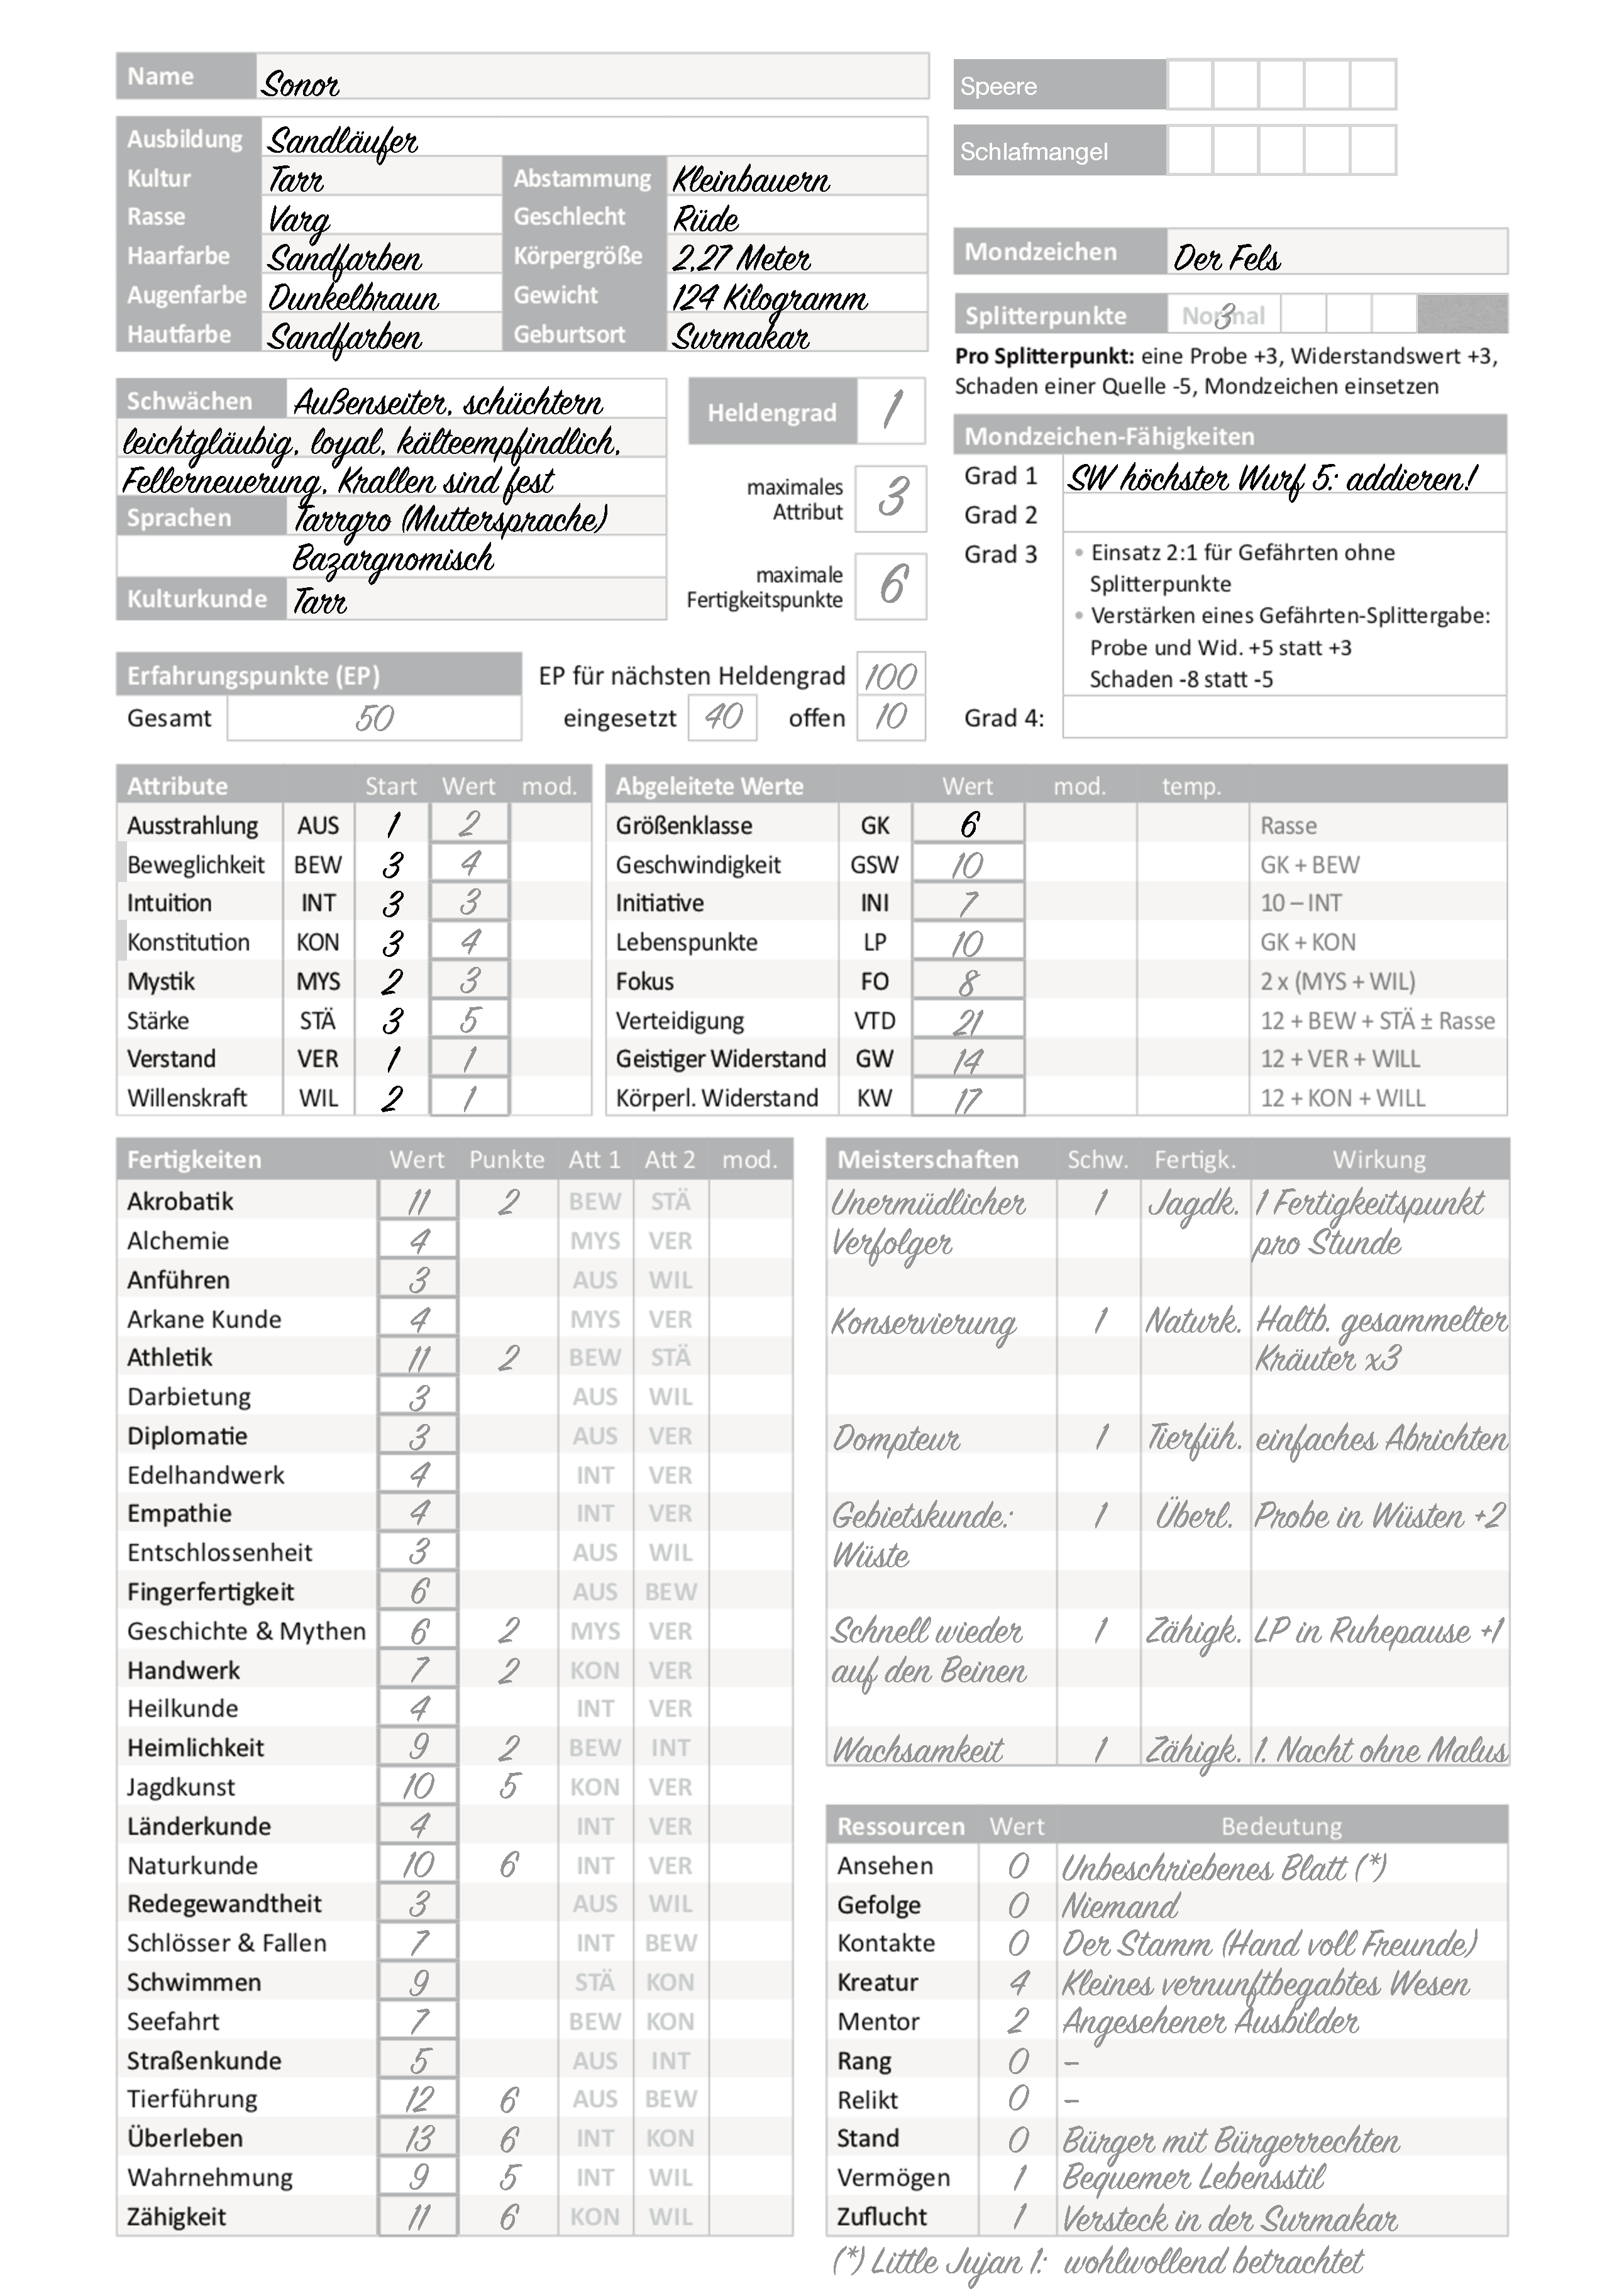
\includepdf[pages=-]{Images/Charakterbogen.pdf}

%% Dokument beenden
\end{document}  